% The contents of this file is 
% Copyright (c) 2009-  Charles R. Severance, All Righs Reserved

\chapter{Programas em redes}
%\chapter{Networked programs}

Enquanto muitos dos exemplos usados neste livro tem focado na leitura de
arquivos e procura por dados neles, existem muitas fontes de informação
diferentes quando se leva em conta a Internet.
%While many of the examples in this book have focused on reading
%files and looking for data in those files, there are many different
%sources of information when one considers the Internet.

Nesse capítulo fingiremos ser um navegador web a obter páginas
web usando o Protocolo de Transferência de Hipertexto ({\it HyperText Transport
Protocol} -- HTTP).  Feito isso, faremos uma leitura
por dados da página web e os analisaremos.
%In this chapter we will pretend to be a web browser and retrieve web
%pages using the HyperText Transport Protocol (HTTP).  Then we will read
%through the web page data and parse it.

\section{Protocolo de Transferência de Hipertexto - HTTP}
%\section{HyperText Transport Protocol - HTTP}

O protocolo de rede que impulsiona a web é, na verdade, bem simples e 
existe um suporte embutido no Python chamado {\tt sockets} que faz com seja
muito fácil estabelecer conexões de rede e obter dados através desses
sockets com um programa Python.
%The network protocol that powers the web is actually quite simple and 
%there is built-in support in Python called {\tt sockets} which makes it very 
%easy to make network connections and retrieve data over those
%sockets in a Python program.

Um {\bf socket} é bem parecido com um arquivo, exceto que um único socket
provê uma conexão de duas vias entre dois programas.  Você pode tanto ler
quanto escrever pelo mesmo socket. Se você escrever alguma coisa em um
socket, a escrita é enviada para a aplicação na outra ponta do socket.
Se você ler a partir de um socket, você está recebendo os dados que a outra
aplicação enviou.
%A {\bf socket} is much like a file, except that a single  socket 
%provides a two-way connection between two programs.  
%You can both read from and write to the same socket.  If you write something to 
%a socket, it is sent to the application at the other end of the socket.  If you 
%read from the socket, you are given the data which the other application has sent.

Mas se você tentar ler um socket enquanto o programa na outra ponta do
socket não enviar nenhum dado---você tem que sentar e esperar.  Se os
programas de ambos os lados do socket simplesmente esperarem por dados sem
enviarem nada, eles continuarão esperando até que alguém envie algum dado..
%But if you try to read a socket when the program on the other end of the socket
%has not sent any data---you just sit and wait.  If the programs on both ends
%of the socket simply wait for some data without sending anything, they will wait for
%a very long time.

Então, uma parte importante dos programas que se comunicam através da Internet
tem algum tipo de protocolo.  Um protocolo é um conjunto de regras precisas
que determinam quem inicia, como será a comunidação, e então quais são as
respostas para a mensagem enviada, e quem envia a próxima, e assim por diante.
De certa forma as aplicações, cada uma em uma ponta do socket, estão dançando e
tem que garantir que uma não vai pisar no pé da outra.
%So an important part of programs that communicate over the Internet is to have some
%sort of protocol.   A protocol is a set of precise rules that determine who
%is to go first, what they are to do, and then what the responses are to that message,
%and who sends next, and so on.  In a sense the two applications at either end 
%of the socket are doing a dance and making sure not to step on each other's toes.

Existem muitos documentos que descrevem estes protocolos de rede. O Protocolo
de Transferência de Hipertexto é descrito no seguinte documento:
%There are many documents which describe these network protocols.  The HyperText Transport 
%Protocol is described in the following document:

\url{http://www.w3.org/Protocols/rfc2616/rfc2616.txt}

Este é um longo e complexo documento de 176 páginas, com muitos detalhes.  Se
você achá-lo interessante, fique à vontade para lê-lo na integra.  Mas se
você der uma olhada pela página 36 do RFC2616, irá encontrar a sintaxe
para a requisição GET. Para requisitar um documento de um servidor web, faremos
uma conexão com o servidor {\tt www.py4inf.com} na porta 80, e então
enviamos uma linha com o seguinte formato:
%This is a long and complex 176-page document with a lot of detail.  If you 
%find it interesting, feel free to read it all.  But if you take a look around page 36 of
%RFC2616 you will find the syntax for the GET request.  To request a document from a web
%server, we make a connection to the {\tt www.py4inf.com} server on port 80, and then
%send a line of the form

{\tt GET http://www.py4inf.com/code/romeo.txt HTTP/1.0 }

onde o segundo parâmetro é a página web que estamos solicitando, e então
enviamos também uma linha em branco. O servidor web irá responder com
algumas informações de cabeçalho sobre o documento e uma linha em branco seguida
do conteúdo do documento.
%where the second parameter is the web page we are requesting, and then 
%we also send a blank line.  The web server will respond with some 
%header information about the document and a blank line
%followed by the document content.

\section{O Navegador Web Mais Simples do Mundo}
%\section{The World's Simplest Web Browser}

Talvez, a maneira mais simples de mostrar como o protocolo HTTP funciona é
escrever um programa Python bem simples que faz a conexão com um servidor web
e segue as regras do protocolo HTTP para solicitar um documento e exibir o
que o servidor envia de volta.
%Perhaps the easiest way to show how the HTTP protocol works is to write a very 
%simple Python program that makes a connection to a web server and follows
%the rules of the HTTP protocol to requests\ a document 
%and display what the server sends back.

\beforeverb
\begin{verbatim}
import socket

mysock = socket.socket(socket.AF_INET, socket.SOCK_STREAM)
mysock.connect(('www.py4inf.com', 80))
mysock.send('GET http://www.py4inf.com/code/romeo.txt HTTP/1.0\n\n')

while True:
    data = mysock.recv(512)
    if ( len(data) < 1 ) :
        break
    print data

mysock.close()
\end{verbatim}
\afterverb

Primeiro, o programa estabelece a conexão na porta 80 do 
servidor \url{www.py4inf.com}. Como nosso programa faz o papel de um 
``navegador web'', o protocolo HTTP informa que nós temos que enviar um comando
GET seguido de uma linha em branco.
%First the program makes a connection to port 80 on 
%the server \url{www.py4inf.com}.
%Since our program is playing the role of the ``web browser'', the HTTP
%protocol says we must send the GET command followed by a blank line.

\beforefig
\centerline{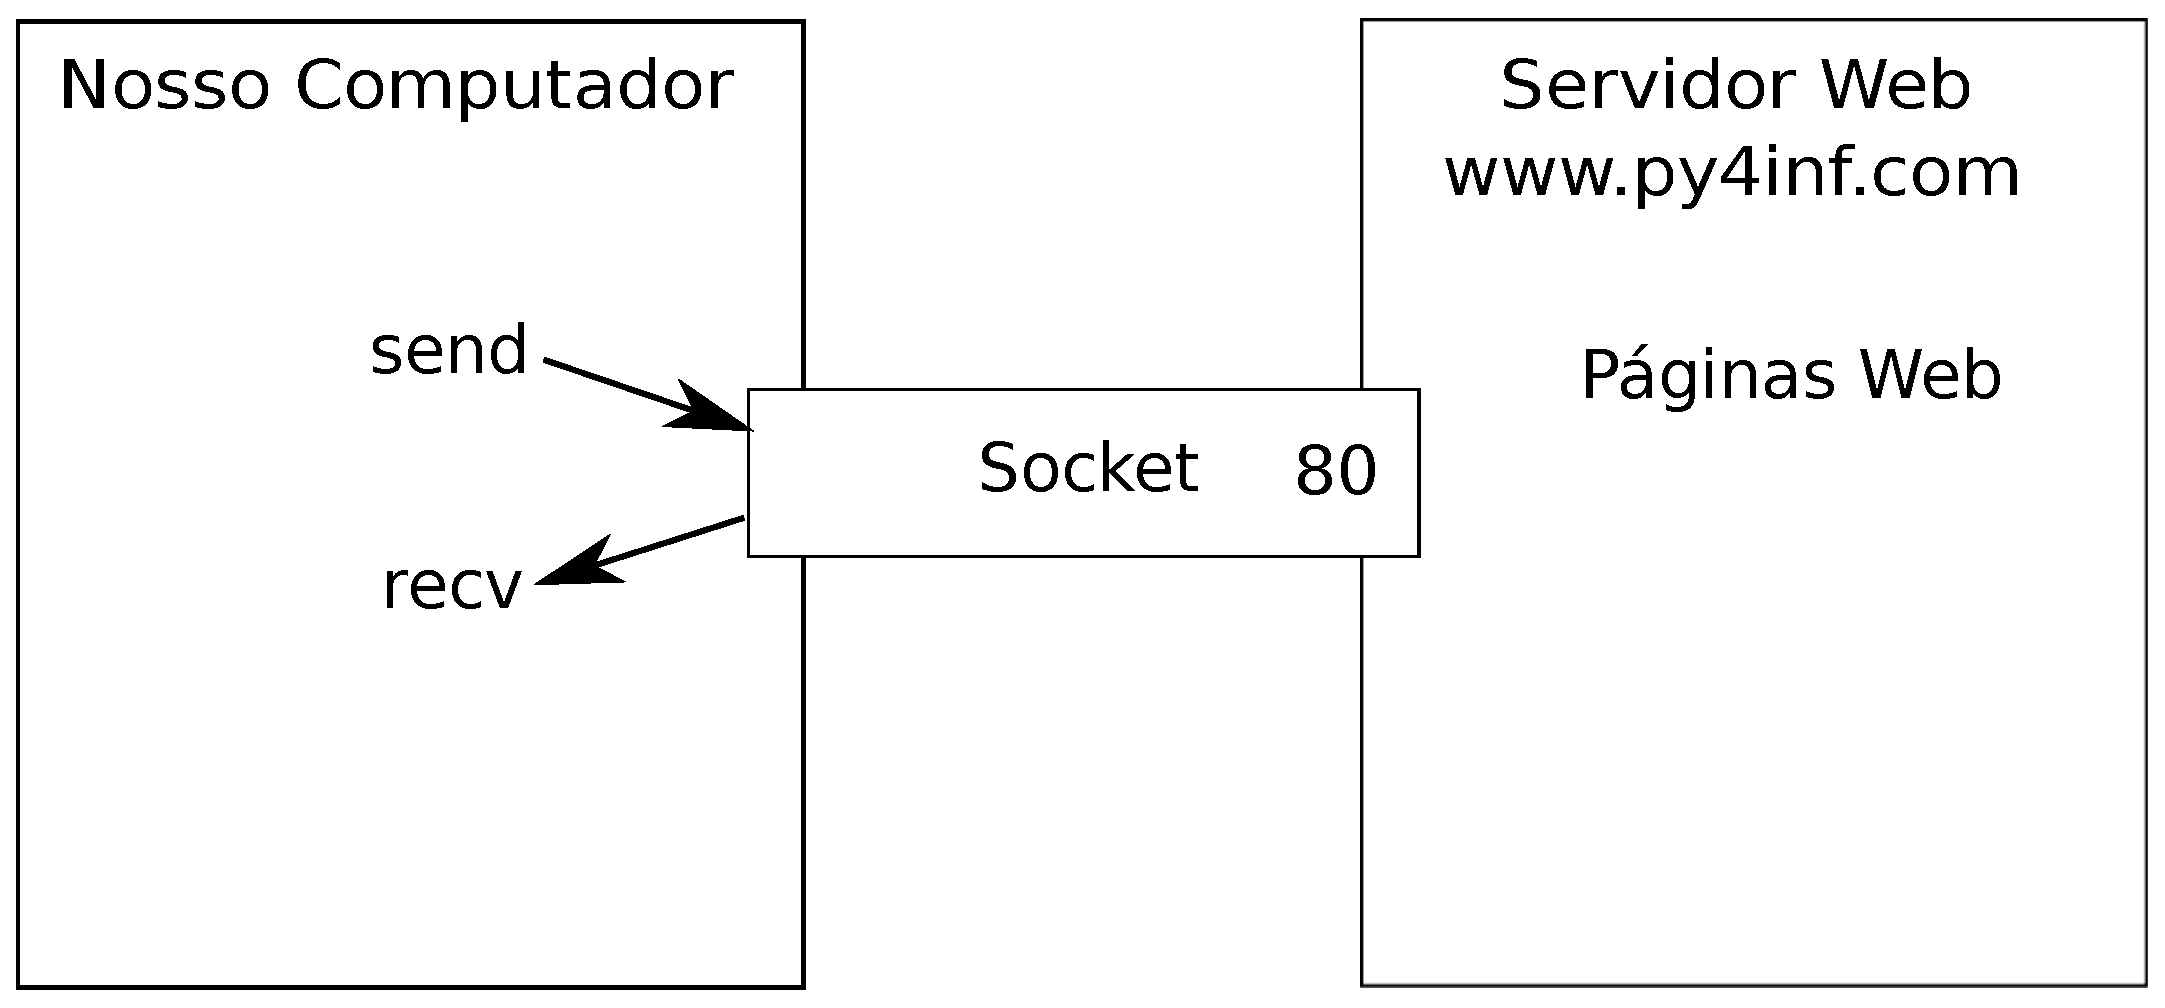
\includegraphics[height=1.50in]{figs2/socket.eps}}
\afterfig

Uma vez enviada a linha em branco, escrevemos um loop que recebe do
socket, dados em pedaços de 512 caracteres e imprime os dados até que não
exista mais dados para ler (por exemplo, a recv() retorna uma string vazia).
%Once we send that blank line, we write a loop that receives data 
%in 512-character chunks from the socket and prints the data out 
%until there is no more data to read (i.e., the recv() returns 
%an empty string).

O programa produz a seguinte saída:
%The program produces the following output:

\beforeverb
\begin{verbatim}
HTTP/1.1 200 OK
Date: Sun, 14 Mar 2010 23:52:41 GMT
Server: Apache
Last-Modified: Tue, 29 Dec 2009 01:31:22 GMT
ETag: "143c1b33-a7-4b395bea"
Accept-Ranges: bytes
Content-Length: 167
Connection: close
Content-Type: text/plain

But soft what light through yonder window breaks
It is the east and Juliet is the sun
Arise fair sun and kill the envious moon
Who is already sick and pale with grief
\end{verbatim}
\afterverb

A saída começa com os cabeçalhos que o servidor web envia para descrever o
documento. Por exemplo, o cabeçalho {\tt Content-Type} indica que o documento
é um documento em texto plano ({\tt text/plain}).
%The output starts with headers which the web server sends
%to describe the document.
%For example, the {\tt Content-Type} header indicates that
%the document is a plain text document ({\tt text/plain}).

Depois que o servidor nos enviar os cabeçalhos, ele adiciona uma linha em branco
para indicar o final dos cabeçalhos, e então, envia realmente os dados do
arquivo {\tt romeo.txt}.
%After the server sends us the headers, it adds a blank line
%to indicate the end of the headers, and then sends the actual
%data of the file {\tt romeo.txt}.

Esse exemplo mostra como fazer uma conexão de rede de baixo nível com sockets.
Sockets podem ser usados para se comunicar com um servidor web ou com um
servidor de e-mail ou muitos outros tipos de servidores. Tudo que é preciso é
encontrar o documento que descreve o protocolo e escrever o código para enviar
e receber os dados de acordo com o protocolo.
%This example shows how to make a low-level network connection
%with sockets.   Sockets can be used to communicate with a web
%server or with a mail server or many other kinds of servers.
%All that is needed is to find the document which describes
%the protocol and write the code to send and receive the data
%according to the protocol.

Contudo, como o protocolo que nós usamos mais  comumente é o protocolo web
HTTP, o Python tem uma biblioteca especificamente desenvolvida para ter suporte
ao protocolo HTTP. E assim, obter documentos e dados através da web.
%However, since the protocol that we use most commonly is
%the HTTP web protocol, Python has a special 
%library specifically designed to support the HTTP protocol 
%for the retrieval of documents and data over the web.

\section{Obtendo uma imagem através do HTTP}
%\section{Retrieving an image over HTTP}

\index{urllib!image}
\index{image!jpg}
\index{jpg}
No exemplo acima, nós pegamos um arquivo em texto plano que tinha novas linhas
dentro do arquivo e nós simplesmente copiamos os dados para a tela a medida
que o programa era executado. Nós podemos usar um programa similar para obter
uma imagem através da web usando o HTTP. Ao invés de copiar os dados para a
tela, a medida que o programa é executado, nós acumulamos os dados em uma
string, retiramos os cabeçalhos, e então salvamos os dados da imagem em um
arquivo. Como a seguir:
%In the above example, we retrieved a plain text file 
%which had newlines in the file and we simply copied the
%data to the screen as the program ran.   We can use a similar
%program to retrieve an image across using HTTP.   Instead
%of copying the data to the screen as the program runs,
%we accumulate the data in a string, trim off the headers,
%and then save the image data to a file as follows:

\beforeverb
\begin{verbatim}
import socket
import time

mysock = socket.socket(socket.AF_INET, socket.SOCK_STREAM)
mysock.connect(('www.py4inf.com', 80))
mysock.send('GET http://www.py4inf.com/cover.jpg HTTP/1.0\n\n')


count = 0
picture = "";
while True:
    data = mysock.recv(5120)
    if ( len(data) < 1 ) : break
    # time.sleep(0.25)
    count = count + len(data)
    print len(data),count
    picture = picture + data

mysock.close()

# Look for the end of the header (2 CRLF)
pos = picture.find("\r\n\r\n");
print 'Header length',pos
print picture[:pos]

# Skip past the header and save the picture data
picture = picture[pos+4:]
fhand = open("stuff.jpg","wb")
fhand.write(picture);
fhand.close()
\end{verbatim}
\afterverb

Quando o programa é executado, ele produz a seguinte saída:
%When the program runs it produces the following output:

\beforeverb
\begin{verbatim}
$ python urljpeg.py 
2920 2920
1460 4380
1460 5840
1460 7300
...
1460 62780
1460 64240
2920 67160
1460 68620
1681 70301
Header length 240
HTTP/1.1 200 OK
Date: Sat, 02 Nov 2013 02:15:07 GMT
Server: Apache
Last-Modified: Sat, 02 Nov 2013 02:01:26 GMT
ETag: "19c141-111a9-4ea280f8354b8"
Accept-Ranges: bytes
Content-Length: 70057
Connection: close
Content-Type: image/jpeg
\end{verbatim}
\afterverb

Você pode ver que para esta url, o cabeçalho {\tt Content-Type} indica que o
corpo do documento é uma imagem ({\tt image/jpeg}). Uma vez terminado o
programa, você pode ver os dados da imagem abrindo o arquivo {\tt stuff.jpg}
com um visualizador de imagens.
%You can see that for this url, the 
%{\tt Content-Type} header indicates that
%body of the document is an image ({\tt image/jpeg}).
%Once the program completes, you can view the image data by opening
%the file {\tt stuff.jpg} in an image viewer.

Durante a execução do programa, você pode ver que não temos 5120 caracteres
para cada vez que chamamos o método {\tt recv()}. Nós pegamos tantos
caracteres quantos foram transferidos através da rede, do servidor web para
nós, no momento que chamamos {\tt recv()}.  Neste exemplo, pegamos 1460 ou 2920
caracteres a cada vez que requisitamos até chegar a 5120 caracteres de dados.
%As the program runs, you can see that we don't get 5120 characters
%each time we call the {\tt recv()} method.
%We get as many characters as have been transferred across the network 
%to us by the web server at the moment we call {\tt recv()}.  
%In this example, we either get 1460 or 2920 characters each time we
%request up to 5120 characters of data.

Os seus resultados podem ser diferentes, dependendo da velocidade de
sua rede.  Note também que na última chamada de {\tt recv()}, nós pegamos
1681 bytes, que é o final do fluxo (stream), e na chamada seguinte da
{\tt recv()} nós recebemos uma string vazia (zero-length). Que nos informa
que o servidor chamou {\tt close()} no seu final de socket e não existe mais
dados para enviar.
%Your results may be different depending on your network speed.  Also
%note that on the last call to {\tt recv()} we get 1681 bytes, which is the end
%of the stream, and in the next call to {\tt recv()} we get a zero-length
%string that tells us that the server has called {\tt close()} on its end 
%of the socket and there is no more data forthcoming.

\index{time}
\index{time.sleep}
Nós podemos reduzir nossas sucessivas chamadas a {\tt recv()} descomentando
, removendo o caractere cerquilha, da chamada de {\tt time.sleep()}.  
Desta forma, nós esperamos
um quarto de segundo depois de cada chamada, e assim, o servidor pode
``se antecipar'' à nós e enviar mais dados antes de nós chamarmos
{\tt recv()} novamente.  Com esse "atraso", o programa é executado
como a seguir:
\beforeverb
\begin{verbatim}
$ python urljpeg.py 
1460 1460
5120 6580
5120 11700
...
5120 62900
5120 68020
2281 70301
Header length 240
HTTP/1.1 200 OK
Date: Sat, 02 Nov 2013 02:22:04 GMT
Server: Apache
Last-Modified: Sat, 02 Nov 2013 02:01:26 GMT
ETag: "19c141-111a9-4ea280f8354b8"
Accept-Ranges: bytes
Content-Length: 70057
Connection: close
Content-Type: image/jpeg
\end{verbatim}
\afterverb

Agora, ao invés de uma primeira e última chamada a {\tt recv()}, nós agora
pegamos 5120 caracteres a cada vez que pedimos novos dados.  
%Now other than the first and last calls to {\tt recv()}, we now get 
%5120 characters each time we ask for new data.  

Existe um buffer entre o servidor, fazendo solicitações {\tt send()} 
e nossa aplicação fazendo solicitações {\tt recv()}.  Quando nós
executamos o programa com o "atraso" estando ativo, em algum momento
o servidor preenche o buffer no socket e é forçado a fazer uma pausa
até que nosso programa comece a esvaziar o buffer.  A pausa, tanto do
envio quanto do recebimento da aplicação, é chamada ``flow control''
(controle de fluxo).
\index{flow control}
%There is a buffer between the server making {\tt send()} requests 
%and our application making {\tt recv()} requests.  When we run the 
%program with the delay in place, at some point the server might 
%fill up the buffer in the socket and be forced to pause until our
%program starts to empty the buffer.  The pausing of either the 
%sending application or the receiving application is called 
%``flow control''.
%\index{flow control}

\section{Obtendo páginas web com {\tt urllib}}
%\section{Retrieving web pages with {\tt urllib}}

Embora nós possamos manualmente enviar e receber dados pelo HTTP 
usando a biblioteca socket, existe uma maneira muito mais simples
de realizar essa tarefa comum em Python pelo uso da biblioteca
{\tt urllib}.
%While we can manually send and receive data over HTTP 
%using the socket library, there is a much simpler way to 
%perform this common task in Python by 
%using the {\tt urllib} library.

Usando a {\tt urllib}, você pode tratar uma página web de maneira muito
parecida a um arquivo. Você simplesmente indica qual página web você
gostaria de obter e a {\tt urllib} lida com todo o protocolo HTTP e detalhes
sobre cabeçalhos.
%Using {\tt urllib},
%you can treat a web page much like a file.   You simply
%indicate which web page you would like to retrieve and
%{\tt urllib} handles all of the HTTP protocol and header 
%details.

O código equivalente para ler o arquivo {\tt romeo.txt} a partir da web usando
a {\tt urllib} é como o seguinte:
%The equivalent code to read the {\tt romeo.txt} file
%from the web using {\tt urllib} is as follows:

\beforeverb
\begin{verbatim}
import urllib

fhand = urllib.urlopen('http://www.py4inf.com/code/romeo.txt')
for line in fhand:
   print line.strip()
\end{verbatim}
\afterverb

Uma vez que a página web tenha sido aberta com {\tt urllib.urlopen}, nós
podemos tratá-la como um arquivo e fazer a leitura usando um loop {\tt for}.
%Once the web page has been opened with 
%{\tt urllib.urlopen}, we can treat it like 
%a file and read through it using a 
%{\tt for} loop.   

Quando o programa é executado, nós apenas vemos na saída o conteúdo do arquivo.
Os cabeçalhos continuam sendo enviados, mas o código da {\tt urllib} consome
os cabeçalhos e apenas retorna os dados para nós.
%When the program runs, we only see the output
%of the contents of the file.   The headers
%are still sent, but the {\tt urllib} code
%consumes the headers and only returns the 
%data to us.

\beforeverb
\begin{verbatim}
But soft what light through yonder window breaks
It is the east and Juliet is the sun
Arise fair sun and kill the envious moon
Who is already sick and pale with grief
\end{verbatim}
\afterverb

Como exemplo, nós podemos escrever um programa para obter os dados de
{\tt romeo.txt} e calcular a frequência de cada palavra existente dentro do
arquivo, como a seguir:
%As an example, we can write 
%a program to retrieve the data for
%{\tt romeo.txt} and compute the frequency
%of each word in the file as follows:

\beforeverb
\begin{verbatim}
import urllib

counts = dict()
fhand = urllib.urlopen('http://www.py4inf.com/code/romeo.txt')
for line in fhand:
    words = line.split()
    for word in words:
        counts[word] = counts.get(word,0) + 1   
print counts
\end{verbatim}
\afterverb

Novamente, uma vez que nós abrimos a página web, podemos fazer a leitura como
um arquivo local.
%Again, once we have opened the web page, 
%we can read it like a local file.

\section{Analizando o HTML e varrendo a web}
\index{web!scraping}
\index{parsing HTML}
%\section{Parsing HTML and scraping the web}
%\index{web!scraping}
%\index{parsing HTML}

Um dos usos comuns da capacidade da {\tt urllib} em Python é 
{\bf varrer} a web. Varrer a web é quando nós escrevemos um programa
que finge ser um navegador web e obtêm páginas, e então examina os dados
nessas páginas a procura de padrões.
%One of the common uses of the {\tt urllib} capability in Python is 
%to {\bf scrape} the web.   Web scraping is when we write a program
%that pretends to be a web browser and retrieves pages, then 
%examines the data in those pages looking for patterns.

Como um exemplo, um mecanismo de busca como o Google irá olhar os fontes de
uma página web e extrair os links para outras páginas e obter essas páginas,
extrair os links para outras páginas e obter essas páginas, extrair links e
assim por diante. Usando essa técnica, o Google {\bf mapeia} seu caminho
através de quase todas as páginas na web.   
%As an example, a search engine such as Google will look at the source 
%of one web page and extract the links to other pages and retrieve
%those pages, extracting links, and so on.   Using this technique,
%Google {\bf spiders} its way through nearly all of the pages on 
%the web.   

O Google também usa a frequência de links das páginas que ele encontra para
uma página em particular de maneira a medir o quão ``importante'' uma página
é, e em que posição a página deve aparecer em seus resultados de pesquisa.
%Google also uses the frequency of links from pages it finds 
%to a particular page as one measure of how ``important'' 
%a page is and how high the page should appear in its search results.

\section{Analisando o HTML através do uso de expressões regulares}
%\section{Parsing HTML using regular expressions}

Uma maneira simples de analisar o HTML é usar expressões regulares, para
repetidamente, buscar e extrair substrings que coincidam com um padrão em
particular.
%One simple way to parse HTML is to use regular expressions to repeatedly
%search for and extract substrings that match a particular pattern.

Aqui está uma página web simples:
%Here is a simple web page:

\beforeverb
\begin{verbatim}
<h1>The First Page</h1>
<p>
If you like, you can switch to the
<a href="http://www.dr-chuck.com/page2.htm">
Second Page</a>.
</p>
\end{verbatim}
\afterverb

Nós podemos construir uma expressão regular para identificar e extrair os
valores dos links do texto abaixo, como a seguir:
%We can construct a well-formed regular expression to match
%and extract the link values from the above text as follows:

\beforeverb
\begin{verbatim}
href="http://.+?"
\end{verbatim}
\afterverb

Nossa expressão regular procura por strings que iniciam com ``href="http://'',
seguida de um ou mais caracteres (``.+?''), seguida por outra aspas. O ponto
de interrogação adicionado ao ``.+?'' indica que a expressão é para coincidir
com um padrão de forma ``não gananciosa'', ao invés de uma maneira
``gananciosa''. Um padrão não ganancioso tenta encontrar a {\em menor} string
correspondente possível e a gananciosa tenta encontrar a {\em maior} string
correspondente possível.
\index{greedy}
\index{non-greedy}
%Our regular expression looks for strings that start with
%``href="http://'', followed by one or more characters
%(``.+?''), followed by another double quote.  The question mark 
%added to the ``.+?'' indicates that the match is to be done
%in a ``non-greedy'' fashion instead of a ``greedy'' fashion.  
%A non-greedy match tries to find the {\em smallest} possible matching
%string and a greedy match tries to find the {\em largest} possible
%matching string.
%\index{greedy}
%\index{non-greedy}

Nós adicionamos parênteses a nossa expressão regular para indicar qual parte
de nossa string correspondente nós gostaríamos de extrair, e foi produzido o
seguinte programa:
\index{regex!parentheses}
\index{parentheses!regular expression}
%We add parentheses to our regular expression to indicate
%which part of our matched string we would like to extract, and
%produce the following program:
%\index{regex!parentheses}
%\index{parentheses!regular expression}

\beforeverb
\begin{verbatim}
import urllib
import re

url = raw_input('Enter - ')
html = urllib.urlopen(url).read()
links = re.findall('href="(http://.*?)"', html)
for link in links:
    print link
\end{verbatim}
\afterverb

O método de expressão regular {\tt findall} irá retornar para nós uma lista
de todas as strings que coincidem com nossa expressão regular, retornando
apenas o texto do link entre as aspas duplas.
%The {\tt findall} regular expression method will give us a list of all
%of the strings that match our regular expression, returning only
%the link text between the double quotes.

Quando nós executamos o programa, nós temos a seguinte saída:
%When we run the program, we get the following output:

\beforeverb
\begin{verbatim}
python urlregex.py 
Enter - http://www.dr-chuck.com/page1.htm
http://www.dr-chuck.com/page2.htm

python urlregex.py 
Enter - http://www.py4inf.com/book.htm
http://www.greenteapress.com/thinkpython/thinkpython.html
http://allendowney.com/
http://www.py4inf.com/code
http://www.lib.umich.edu/espresso-book-machine
http://www.py4inf.com/py4inf-slides.zip
\end{verbatim}
\afterverb

As expressões regulares funcionam muito bem quando o seu HTML está bem
formatado e previsível.  Mas como existem muitas páginas HTML ``quebradas''
por aí, a solução usando expressões regulares pode perder alguns links
válidos ou terminar com dados ruins.
%Regular expressions work very nicely when your HTML is well formatted
%and predictable.  But since there are a lot of ``broken'' HTML pages
%out there, a solution only using regular expressions might either miss
%some valid links or end up with bad data.

Isso pode ser resolvido utilizando uma robusta biblioteca de análise de HTML.
%This can be solved by using a robust HTML parsing library.

\section{Analisando o HTML com o uso da BeautifulSoup}
%\section{Parsing HTML using BeautifulSoup}
%\index{BeautifulSoup}

Existem várias bibliotecas Python que podem ajudar você a analisar o HTML e
extrair dados das páginas. Cada uma das bibliotecas tem suas vantagens e
desvantagens e você pode escolher uma com base em suas necessidades.
%There are a number of Python libraries which can help you parse
%HTML and extract data from the pages.  Each of the libraries
%has its strengths and weaknesses and you can pick one based on 
%your needs.

Como exemplo, iremos simplesmente analisar alguma entrada HTML e extrair os
links usando a biblioteca {\bf BeautifulSoup}. Você pode baixar e instalar o
código BeautifulSoup de:
%As an example, we will simply parse some HTML input 
%and extract links using the {\bf BeautifulSoup} library.   
%You can download and install the BeautifulSoup code
%from:

\url{http://www.crummy.com/software/}

Você pode baixar e fazer a ``instalação'' da biblioteca BeautifulSoup ou pode
simplesmente colocar o arquivo {\tt BeautifulSoup.py} no mesmo diretório que
está a sua aplicação.
%You can download and ``install'' BeautifulSoup or you 
%can simply place the {\tt BeautifulSoup.py} file in the
%same folder as your application.

Ainda que o HTML se pareça com XML\footnote{O formato XML será descrito no
próximo capítulo.} e algumas páginas são cuidadosamente construídas para ser
um XML, a maioria do HTML é, geralmente, quebrado. O que faz com que um
analisador XML rejeite toda a página HTML por concluir que ela está
impropriamente formada. A BeautifulSoup tolera muitas imperfeições HTML e
ainda permite que você extraia facilmente os dados que você precisa.
%Even though HTML looks like XML\footnote{The XML format is described in
%the next chapter.} and some pages are carefully 
%constructed to be XML, most HTML is generally broken in ways
%that cause an XML parser to reject the entire page of HTML as
%improperly formed.  BeautifulSoup tolerates highly flawed 
%HTML and still lets you easily extract the data you need.

Nós iremos usar a {\tt urllib} para ler a página e então usar a
{\tt BeautifulSoup} para extrair os atributos {\tt href} das tags de ancoragem
({\tt a}).
\index{BeautifulSoup}
\index{HTML}
\index{parsing!HTML}
%We will use {\tt urllib} to read the page and then use
%{\tt BeautifulSoup} to extract the {\tt href} attributes from the
%anchor ({\tt a}) tags.
%\index{BeautifulSoup}
%\index{HTML}
%\index{parsing!HTML}

\beforeverb
\begin{verbatim}
import urllib
from BeautifulSoup import *

url = raw_input('Enter - ')
html = urllib.urlopen(url).read()
soup = BeautifulSoup(html)

# Retrieve all of the anchor tags
tags = soup('a')
for tag in tags:
   print tag.get('href', None)
\end{verbatim}
\afterverb

O programa pede um endereço web, e então abre a página web, lê os dados e
passa os dados para o analisador BeautifulSoup, e então obtém todas as tags
de ancoragem e imprime o atributo {\tt href} de cada tag.
%The program prompts for a web address, then opens the web
%page, reads the data and passes the data to the BeautifulSoup
%parser, and then retrieves all of the anchor tags and prints
%out the {\tt href} attribute for each tag.

Quando o programa é executado, ele se parece como a seguir:
%When the program runs it looks as follows:

\beforeverb
\begin{verbatim}
python urllinks.py 
Enter - http://www.dr-chuck.com/page1.htm
http://www.dr-chuck.com/page2.htm

python urllinks.py 
Enter - http://www.py4inf.com/book.htm
http://www.greenteapress.com/thinkpython/thinkpython.html
http://allendowney.com/
http://www.si502.com/
http://www.lib.umich.edu/espresso-book-machine
http://www.py4inf.com/code
http://www.pythonlearn.com/
\end{verbatim}
\afterverb

Você pode usar a BeautifulSoup para buscar várias partes de cada tag como a
seguir:
%You can use BeautifulSoup to pull out various parts of each 
%tag as follows:

\beforeverb
\begin{verbatim}
import urllib
from BeautifulSoup import *

url = raw_input('Enter - ')
html = urllib.urlopen(url).read()
soup = BeautifulSoup(html)

# Retrieve all of the anchor tags
tags = soup('a')
for tag in tags:
   # Look at the parts of a tag
   print 'TAG:',tag
   print 'URL:',tag.get('href', None)
   print 'Content:',tag.contents[0]
   print 'Attrs:',tag.attrs
\end{verbatim}
\afterverb

Isso produz a seguinte saída:
%This produces the following output:

\beforeverb
\begin{verbatim}
python urllink2.py 
Enter - http://www.dr-chuck.com/page1.htm
TAG: <a href="http://www.dr-chuck.com/page2.htm">
Second Page</a>
URL: http://www.dr-chuck.com/page2.htm
Content: [u'\nSecond Page']
Attrs: [(u'href', u'http://www.dr-chuck.com/page2.htm')]
\end{verbatim}
\afterverb

Estes exemplos apenas começam a mostrar o poder da BeautifulSoup, quando se
refere a análise de HTML. Veja a documentação e exemplos em
\url{http://www.crummy.com/software/BeautifulSoup/} para mais detalhes.
%These examples only begin to show the power of BeautifulSoup
%when it comes to parsing HTML.  See the documentation 
%and samples at
%\url{http://www.crummy.com/software/BeautifulSoup/} for more detail.

\section{Lendo arquivos binários usando a {\tt urllib}}
%\section{Reading binary files using urllib}

Algumas vezes, você quer obter um arquivo não texto (ou binário), como um
arquivo de imagem ou vídeo. Os dados nesses arquivos geralmente não são úteis
para serem impressos, mas você pode facilmente fazer uma cópia da URL para um
arquivo local em seu disco rígido usando a {\tt urllib}.
\index{binary file}
%Sometimes you want to retrieve a non-text (or binary) file such as
%an image or video file. The data in these files is generally not 
%useful to print out, but you can easily make a copy of a URL to a local
%file on your hard disk using {\tt urllib}.
%\index{binary file}

O padrão é abrir a URL e usar {\tt read} para baixar o conteúdo completo do
documento para dentro de uma variável string ({\tt img}), e então escrever
essa informação em um arquivo local, como a seguir:
%The pattern is to open the URL and use {\tt read} to download the entire
%contents of the document into a string variable ({\tt img}) then write that
%information to a local file as follows:

\beforeverb
\begin{verbatim}
img = urllib.urlopen('http://www.py4inf.com/cover.jpg').read()
fhand = open('cover.jpg', 'w')
fhand.write(img)
fhand.close()
\end{verbatim}
\afterverb

Esse programa lê todos os dados, de uma vez, através da rede e os armazena
dentro da variável {\tt img}, na memória de seu, computador. Então abre o
arquivo {\tt cover.jpg} e escreve os dados para o seu disco.  Isso irá
funcionar se o tamanho do arquivo for menor que o tamanho da memória de seu
computador.
%This program reads all of the data in at once across the network and 
%stores it in the variable {\tt img} in the main memory of your computer,
%then opens the file {\tt cover.jpg} and writes the data out to your 
%disk.  This will work if the size of the file is less than the size
%of the memory of your computer.

Contudo, se ele for um arquivo de áudio ou vídeo grande, esse programa pode
falhar ou pelo menos rodar de forma extremamente vagarosa quando seu computador
ficar sem memória.  Para evitar este tipo de problema, nós podemos obter os
dados em blocos (ou buffers) e então escrever cada bloco no disco antes de
obter o próximo bloco.  Desta forma o programa pode ler um arquivo de qualquer
tamanho sem usar toda a memória que você tem em seu computador.
%However if this is a large audio or video file, this program may crash
%or at least run extremely slowly when your computer runs out of memory.
%In order to avoid running out of memory, we retrieve the data in blocks
%(or buffers) and then write each block to your disk before retrieving
%the next block.  This way the program can read any size file without
%using up all of the memory you have in your computer.

\beforeverb
\begin{verbatim}
import urllib

img = urllib.urlopen('http://www.py4inf.com/cover.jpg')
fhand = open('cover.jpg', 'w')
size = 0
while True:
    info = img.read(100000)
    if len(info) < 1 : break
    size = size + len(info)
    fhand.write(info)

print size,'characters copied.'
fhand.close()
\end{verbatim}
\afterverb

Neste exemplo, nós lemos apenas 100,000 caracteres por vez e então escrevemos
esses caracteres no arquivo {\tt cover.jpg} antes de obter os próximos 100,000
caracteres de dados a partir da web.
%In this example, we read only 100,000 characters at a time and then 
%write those characters to the {\tt cover.jpg} file
%before retrieving the next 100,000 characters of data from the
%web.

Esse programa é executado como a seguir:
%This program runs as follows:

\beforeverb
\begin{verbatim}
python curl2.py 
568248 characters copied.
\end{verbatim}
\afterverb

Se você tem um computador Unix ou Macintosh, você provavelmente tem um comando
em seu sistema operacional que executa essa operação, como a seguir:
\index{curl}
%If you have a Unix or Macintosh computer, you probably have a command
%built in to your operating system that performs this operation
%as follows:
%\index{curl}

\beforeverb
\begin{verbatim}
curl -O http://www.py4inf.com/cover.jpg
\end{verbatim}
\afterverb

O comando {\tt curl} é a abreviação para ``copy URL'', então esses dois
exemplos são, inteligentemente, chamados de {\tt curl1.py} e {\tt curl2.py} em
\url{www.py4inf.com/code}, já que eles implementam uma funcionalidade similar
ao comando {\tt curl}.  Existe também um programa exemplo {\tt curl3.py} que
realiza essa tarefa de maneira um pouco mais efetiva, caso você queira
realmente usar esse padrão em um programa que esteja escrevendo.
%The command {\tt curl} is short for ``copy URL'' and so these two 
%examples are cleverly named {\tt curl1.py} and {\tt curl2.py} on 
%\url{www.py4inf.com/code} as they implement similar functionality
%to the {\tt curl} command.  There is also a {\tt curl3.py} sample 
%program that does this task a little more effectively, in case you
%actually want to use this pattern in a program you are writing.

\section{Glossário}
%\section{Glossary}

\begin{description}
%\begin{description}

\item[BeautifulSoup:] Uma biblioteca Python para análise de documentos HTML e
extração de dados desses documentos HTML que faz compensações nas maiorias das
imperfeições em um HTML que os navegadores geralmente ignoram. Você pode
baixar o código da BeautifulSoup em \url{www.crummy.com}.
\index{BeautifulSoup}
%\item[BeautifulSoup:] A Python library for parsing HTML documents
%and extracting data from HTML documents
%that compensates for most of the imperfections in the HTML that browsers
%generally ignore.
%You can download the BeautifulSoup code
%from 
%\url{www.crummy.com}.
%\index{BeautifulSoup}

\item[porta:] Um número que geralmente indica qual aplicação você está
contactando quando você faz uma conexão por socket com um servidor. Como um
exemplo, o tráfego web, usualmente, usa a porta 80, enquanto o tráfego de
e-mail usa a porta 25.
\index{port}
%\item[port:] A number that generally indicates which application 
%you are contacting when you make a socket connection to a server.
%As an example, web traffic usually uses port 80 while email 
%traffic uses port 25.
%\index{port}

\item[scraping:] Quando um programa finge ser um navegador web, obtém uma página
web, e então olha o conteúdo da página web. Geralmente os programas estão
seguindo os links de uma página para encontrar a próxima página. Para que
eles possam atravessar uma rede de páginas ou uma rede social.
\index{web!scraping}
%\item[scrape:] When a program pretends to be a web browser and
%retrieves a web page, then looks at the web page content. 
%Often programs are following the links in one page to find the next
%page so they can traverse a network of pages or a social network.
%\index{socket}

\item[socket:] Uma conexão de rede entre duas aplicações. Onde as aplicações
podem enviar e receber dados em ambas as direções.
\index{socket}
%\item[socket:] A network connection between two applications
%where the applications can send and receive data in either direction.
%\index{socket}

\item[spider:] Um mecanismo que busca pela web obtendo uma página e então todas
as páginas com ligações a partir dessa página e assim por diante até ele ter
praticamente todas as páginas na Internet que ele usará para construir sua
indexação de busca.
\index{spider}
%\item[spider:] The act of a web search engine retrieving a page and
%then all the pages linked from a page and so on until they have 
%nearly all of the pages on the Internet which they 
%use to build their search index.
%\index{spider}

\end{description}
%\end{description}

\section{Exercícios}
%\section{Exercises}

\begin{ex}
Altere o programa socket {\tt socket1.py} para pedir ao usuário a URL, e assim,
ele possa ler qualquer página web. Você pode usar {\tt split('/')} para quebrar
a URL em partes de componentes para que você possa extrair o nome da máquina
para a chamada {\tt connect}. Adicionar uma checagem de erro usando {\tt try}
e {\tt except} para lidar com a conexão, caso o usuário digite um formato de
URL impróprio ou não existente.  
\end{ex}
%\begin{ex}
%Change the socket program {\tt socket1.py} to prompt the user for 
%the URL so it can read any web page.  
%You can use {\tt split('/')} to break the URL into its component parts
%so you can extract the host name for the socket {\tt connect} call.
%Add error checking using {\tt try} and {\tt except} to handle the condition where the 
%user enters an improperly formatted or non-existent URL.  
%\end{ex}

\begin{ex}
Altere seu programa socket para que ele conte o número de caracteres que ele
tenha recebido e interrompa a exibição de qualquer texto após ele ter mostrado
3000 caracteres.  O programa deve obter o documento por inteiro, contar o
número total de caracteres e exibir a contagem do número de caracteres no
final do documento.
\end{ex}
%\begin{ex}
%Change your socket program so that it counts the number of characters it has received 
%and stops displaying any text after it has shown 3000 characters.  The program 
%should retrieve the entire document and count the total number of characters 
%and display the count of the number of characters at the end of the document.
%\end{ex}

\begin{ex}
Use a {\tt urllib} para replicar o exercício prévio de (1) obtenção de um
documento a partir de uma URL, (2) exibindo até 3000 caracteres, e (3)
desfazendo a contagem do total de caracteres no documento.  Não se preocupe
com os cabeçalhos neste exercício, apenas mostre os primeiros 3000 caracteres
do conteúdo do documento.
\end{ex}
%\begin{ex}
%Use {\tt urllib} to replicate the previous exercise of (1) retrieving the document
%from a URL, (2) displaying up to 3000 characters, and (3) counting the overall number
%of characters in the document.  Don't worry about the headers for this exercise, simply
%show the first 3000 characters of the document contents.
%\end{ex}

\begin{ex}
Altere o programa {\tt urllinks.py} para que ele extraia e conte as tags
parágrafo (p) de um documento HTML obtido e exiba a contagem de parágrafos
como saída de seu programa. Não exiba o texto de parágrafo, apenas faça a
contagem. Teste seu programa em várias páginas web pequenas. E também em
algumas páginas web grandes.
\end{ex}
%\begin{ex}
%Change the {\tt urllinks.py} program to extract and count 
%paragraph (p) tags from the retrieved HTML document and 
%display the count of the paragraphs as the 
%output of your program.  
%Do not display the paragraph text, only count them.
%Test your program on several small web pages
%as well as some larger web pages.
%\end{ex}

\begin{ex}
(Avançado) Altere o programa socket para que ele apenas mostre os dados
após os cabeçalhos até que uma linha em branco tenha sido recebida. Lembre 
que o {\tt recv} está recebendo caracteres (nova linha e outros caracteres),
não linhas.
\end{ex}
%\begin{ex}
%(Advanced) Change the socket program so that it only shows data after the 
%headers and a blank line have been received.  Remember that {\tt recv} is
%receiving characters (newlines and all), not lines.
%\end{ex}
